\subsection{Problem}
\renewcommand{\theequation}{\theenumi}
\begin{enumerate}[label=\thesection.\arabic*.,ref=\thesection.\theenumi]
\numberwithin{equation}{enumi}

\item Three coins are tossed simultaneously. Consider the event E ”three heads or three tails”, F ”at least two heads” and G ”at most two heads”. Of the pairs (E,F), (E,G) and (F,G), which are independent? which are dependent?\\

\solution The sample size = Possible number of tosses=8
\begin{align}
\resizebox{\columnwidth}{!}{%
\myvec{\bmat{HHH}&\bmat{TTT}&\bmat{HHT}&\bmat{HTT}&\bmat{HTH}&\bmat{TTH}\bmat{THT}&\bmat{THH}}
}
\end{align}
Favourable outcome for event E = three Heads (or) three Tails
\begin{align}
\myvec{\bmat{HHH}&\bmat{TTT}}
\end{align}

\begin{align}
P\brak{E} = \frac{1}{4}
\end{align}


Favourable outcome for event F = atleast two Heads 
\begin{align}
\resizebox{\columnwidth}{!}{%
\myvec{\bmat{HHT}&\bmat{HHH}&\bmat{HTH}&\bmat{THH}}
}
\end{align}

\begin{align}
P\brak{F} = \frac{1}{2}
\end{align}

Favourable outcome for event G = atmost two Heads
\begin{align}
\resizebox{\columnwidth}{!}{%
\myvec{\bmat{TTT}&\bmat{HHT}&\bmat{HTT}&\bmat{HTH}&\bmat{TTH}\bmat{THT}&\bmat{THH}}
}
\end{align}



\begin{align}
P\brak{G} = \frac{7}{8}
\end{align}


Favourable outcome for event E$\cap$F
\begin{align}
\myvec{\bmat{HHH}}
\end{align}

\begin{align}
P\brak{E\cap F} = \frac{1}{8}
\end{align}


Favourable outcome for event F$\cap$G 
\begin{align}
\myvec{\bmat{HHH}&\bmat{HTH}&\bmat{THH}}
\end{align}

\begin{align}
P\brak{F\cap G} = \frac{3}{8}
\end{align}

Favourable outcome for event E$\cap$G
\begin{align}
\myvec{\bmat{TTT}}
\end{align}



\begin{align}
P\brak{E\cap G} = \frac{1}{8}
\end{align}

From the above equations we see that\\
\begin{align}
P\brak{E\cap F} = P\brak{E}.P\brak{F}\\
P\brak{G\cap F} \neq P\brak{G}.P\brak{F}\\
P\brak{E\cap G} \neq P\brak{E}.P\brak{G}
\end{align}
Hence only the pair (E,F) are independent events. The pairs (F,G) and (G,E) are dependent events.
\begin{comment}
	\begin{lstlisting}
	./codes/triangle/q2.py
	\end{lstlisting}
	
	\begin{figure}[!ht]
	\centering
	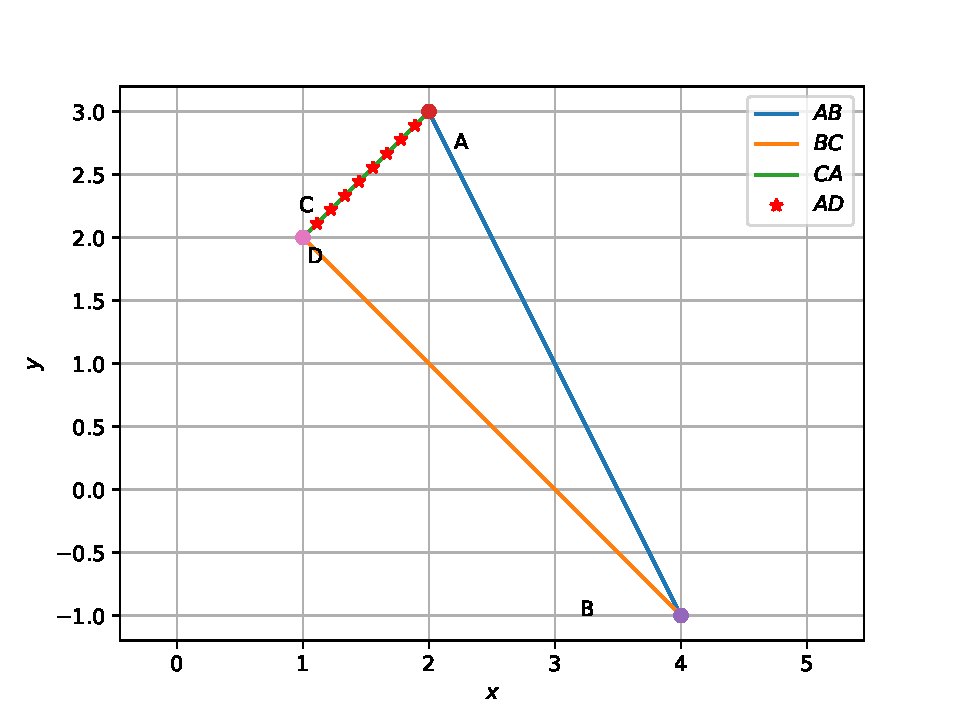
\includegraphics[width=\columnwidth]{./figs/triangle/q2.pdf}
	\caption{Triangle of Q.1.2.5}
	\label{fig:qtwo}	
	\end{figure}
	

\end{comment}	
	
	
\end{enumerate}
